\documentclass[1p]{elsarticle_modified}
%\bibliographystyle{elsarticle-num}

%\usepackage[colorlinks]{hyperref}
%\usepackage{abbrmath_seonhwa} %\Abb, \Ascr, \Acal ,\Abf, \Afrak
\usepackage{amsfonts}
\usepackage{amssymb}
\usepackage{amsmath}
\usepackage{amsthm}
\usepackage{scalefnt}
\usepackage{amsbsy}
\usepackage{kotex}
\usepackage{caption}
\usepackage{subfig}
\usepackage{color}
\usepackage{graphicx}
\usepackage{xcolor} %% white, black, red, green, blue, cyan, magenta, yellow
\usepackage{float}
\usepackage{setspace}
\usepackage{hyperref}

\usepackage{tikz}
\usetikzlibrary{arrows}

\usepackage{multirow}
\usepackage{array} % fixed length table
\usepackage{hhline}

%%%%%%%%%%%%%%%%%%%%%
\makeatletter
\renewcommand*\env@matrix[1][\arraystretch]{%
	\edef\arraystretch{#1}%
	\hskip -\arraycolsep
	\let\@ifnextchar\new@ifnextchar
	\array{*\c@MaxMatrixCols c}}
\makeatother %https://tex.stackexchange.com/questions/14071/how-can-i-increase-the-line-spacing-in-a-matrix
%%%%%%%%%%%%%%%

\usepackage[normalem]{ulem}

\newcommand{\msout}[1]{\ifmmode\text{\sout{\ensuremath{#1}}}\else\sout{#1}\fi}
%SOURCE: \msout is \stkout macro in https://tex.stackexchange.com/questions/20609/strikeout-in-math-mode

\newcommand{\cancel}[1]{
	\ifmmode
	{\color{red}\msout{#1}}
	\else
	{\color{red}\sout{#1}}
	\fi
}

\newcommand{\add}[1]{
	{\color{blue}\uwave{#1}}
}

\newcommand{\replace}[2]{
	\ifmmode
	{\color{red}\msout{#1}}{\color{blue}\uwave{#2}}
	\else
	{\color{red}\sout{#1}}{\color{blue}\uwave{#2}}
	\fi
}

\newcommand{\Sol}{\mathcal{S}} %segment
\newcommand{\D}{D} %diagram
\newcommand{\A}{\mathcal{A}} %arc


%%%%%%%%%%%%%%%%%%%%%%%%%%%%%5 test

\def\sl{\operatorname{\textup{SL}}(2,\Cbb)}
\def\psl{\operatorname{\textup{PSL}}(2,\Cbb)}
\def\quan{\mkern 1mu \triangleright \mkern 1mu}

\theoremstyle{definition}
\newtheorem{thm}{Theorem}[section]
\newtheorem{prop}[thm]{Proposition}
\newtheorem{lem}[thm]{Lemma}
\newtheorem{ques}[thm]{Question}
\newtheorem{cor}[thm]{Corollary}
\newtheorem{defn}[thm]{Definition}
\newtheorem{exam}[thm]{Example}
\newtheorem{rmk}[thm]{Remark}
\newtheorem{alg}[thm]{Algorithm}

\newcommand{\I}{\sqrt{-1}}
\begin{document}

%\begin{frontmatter}
%
%\title{Boundary parabolic representations of knots up to 8 crossings}
%
%%% Group authors per affiliation:
%\author{Yunhi Cho} 
%\address{Department of Mathematics, University of Seoul, Seoul, Korea}
%\ead{yhcho@uos.ac.kr}
%
%
%\author{Seonhwa Kim} %\fnref{s_kim}}
%\address{Center for Geometry and Physics, Institute for Basic Science, Pohang, 37673, Korea}
%\ead{ryeona17@ibs.re.kr}
%
%\author{Hyuk Kim}
%\address{Department of Mathematical Sciences, Seoul National University, Seoul 08826, Korea}
%\ead{hyukkim@snu.ac.kr}
%
%\author{Seokbeom Yoon}
%\address{Department of Mathematical Sciences, Seoul National University, Seoul, 08826,  Korea}
%\ead{sbyoon15@snu.ac.kr}
%
%\begin{abstract}
%We find all boundary parabolic representation of knots up to 8 crossings.
%
%\end{abstract}
%\begin{keyword}
%    \MSC[2010] 57M25 
%\end{keyword}
%
%\end{frontmatter}

%\linenumbers
%\tableofcontents
%
\newcommand\colored[1]{\textcolor{white}{\rule[-0.35ex]{0.8em}{1.4ex}}\kern-0.8em\color{red} #1}%
%\newcommand\colored[1]{\textcolor{white}{ #1}\kern-2.17ex	\textcolor{white}{ #1}\kern-1.81ex	\textcolor{white}{ #1}\kern-2.15ex\color{red}#1	}

{\Large $\underline{12a_{0440}~(K12a_{0440})}$}

\setlength{\tabcolsep}{10pt}
\renewcommand{\arraystretch}{1.6}
\vspace{1cm}\begin{tabular}{m{100pt}>{\centering\arraybackslash}m{274pt}}
\multirow{5}{120pt}{
	\centering
	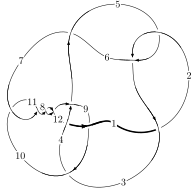
\includegraphics[width=112pt]{../../../GIT/diagram.site/Diagrams/png/1241_12a_0440.png}\\
\ \ \ A knot diagram\footnotemark}&
\allowdisplaybreaks
\textbf{Linearized knot diagam} \\
\cline{2-2}
 &
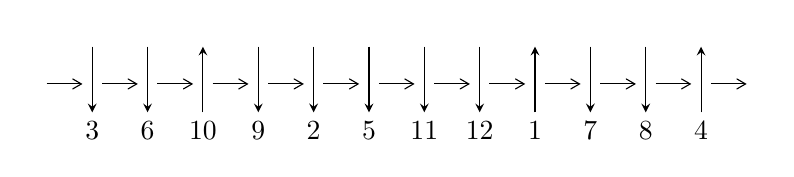
\begin{tikzpicture}[x=20pt, y=17pt]
	% nodes
	\node (C0) at (0, 0) {};
	\node (C1) at (1, 0) {};
	\node (C1U) at (1, +1) {};
	\node (C1D) at (1, -1) {3};

	\node (C2) at (2, 0) {};
	\node (C2U) at (2, +1) {};
	\node (C2D) at (2, -1) {6};

	\node (C3) at (3, 0) {};
	\node (C3U) at (3, +1) {};
	\node (C3D) at (3, -1) {10};

	\node (C4) at (4, 0) {};
	\node (C4U) at (4, +1) {};
	\node (C4D) at (4, -1) {9};

	\node (C5) at (5, 0) {};
	\node (C5U) at (5, +1) {};
	\node (C5D) at (5, -1) {2};

	\node (C6) at (6, 0) {};
	\node (C6U) at (6, +1) {};
	\node (C6D) at (6, -1) {5};

	\node (C7) at (7, 0) {};
	\node (C7U) at (7, +1) {};
	\node (C7D) at (7, -1) {11};

	\node (C8) at (8, 0) {};
	\node (C8U) at (8, +1) {};
	\node (C8D) at (8, -1) {12};

	\node (C9) at (9, 0) {};
	\node (C9U) at (9, +1) {};
	\node (C9D) at (9, -1) {1};

	\node (C10) at (10, 0) {};
	\node (C10U) at (10, +1) {};
	\node (C10D) at (10, -1) {7};

	\node (C11) at (11, 0) {};
	\node (C11U) at (11, +1) {};
	\node (C11D) at (11, -1) {8};

	\node (C12) at (12, 0) {};
	\node (C12U) at (12, +1) {};
	\node (C12D) at (12, -1) {4};
	\node (C13) at (13, 0) {};

	% arrows
	\draw[->,>={angle 60}]
	(C0) edge (C1) (C1) edge (C2) (C2) edge (C3) (C3) edge (C4) (C4) edge (C5) (C5) edge (C6) (C6) edge (C7) (C7) edge (C8) (C8) edge (C9) (C9) edge (C10) (C10) edge (C11) (C11) edge (C12) (C12) edge (C13) ;	\draw[->,>=stealth]
	(C1U) edge (C1D) (C2U) edge (C2D) (C3D) edge (C3U) (C4U) edge (C4D) (C5U) edge (C5D) (C6U) edge (C6D) (C7U) edge (C7D) (C8U) edge (C8D) (C9D) edge (C9U) (C10U) edge (C10D) (C11U) edge (C11D) (C12D) edge (C12U) ;
	\end{tikzpicture} \\
\hhline{~~} \\& 
\textbf{Solving Sequence} \\ \cline{2-2} 
 &
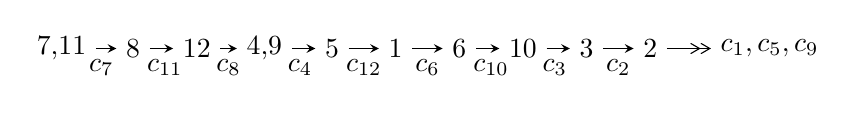
\begin{tikzpicture}[x=23pt, y=7pt]
	% node
	\node (A0) at (-1/8, 0) {7,11};
	\node (A1) at (1, 0) {8};
	\node (A2) at (2, 0) {12};
	\node (A3) at (49/16, 0) {4,9};
	\node (A4) at (33/8, 0) {5};
	\node (A5) at (41/8, 0) {1};
	\node (A6) at (49/8, 0) {6};
	\node (A7) at (57/8, 0) {10};
	\node (A8) at (65/8, 0) {3};
	\node (A9) at (73/8, 0) {2};
	\node (C1) at (1/2, -1) {$c_{7}$};
	\node (C2) at (3/2, -1) {$c_{11}$};
	\node (C3) at (5/2, -1) {$c_{8}$};
	\node (C4) at (29/8, -1) {$c_{4}$};
	\node (C5) at (37/8, -1) {$c_{12}$};
	\node (C6) at (45/8, -1) {$c_{6}$};
	\node (C7) at (53/8, -1) {$c_{10}$};
	\node (C8) at (61/8, -1) {$c_{3}$};
	\node (C9) at (69/8, -1) {$c_{2}$};
	\node (A10) at (11, 0) {$c_{1},c_{5},c_{9}$};

	% edge
	\draw[->,>=stealth]	
	(A0) edge (A1) (A1) edge (A2) (A2) edge (A3) (A3) edge (A4) (A4) edge (A5) (A5) edge (A6) (A6) edge (A7) (A7) edge (A8) (A8) edge (A9) ;
	\draw[->>,>={angle 60}]	
	(A9) edge (A10);
\end{tikzpicture} \\ 

\end{tabular} \\

\footnotetext{
The image of knot diagram is generated by the software ``\textbf{Draw programme}" developed by Andrew Bartholomew(\url{http://www.layer8.co.uk/maths/draw/index.htm\#Running-draw}), where we modified some parts for our purpose(\url{https://github.com/CATsTAILs/LinksPainter}).
}\phantom \\ \newline 
\centering \textbf{Ideals for irreducible components\footnotemark of $X_{\text{par}}$} 
 
\begin{align*}
I^u_{1}&=\langle 
8.17973\times10^{78} u^{78}-3.32534\times10^{79} u^{77}+\cdots+1.08264\times10^{78} b+1.17493\times10^{79},\\
\phantom{I^u_{1}}&\phantom{= \langle  }7.38204\times10^{76} u^{78}+1.20719\times10^{79} u^{77}+\cdots+2.16527\times10^{78} a-2.53946\times10^{79},\;u^{79}-5 u^{78}+\cdots+9 u-1\rangle \\
I^u_{2}&=\langle 
b,\;a^3+a^2+2 a+1,\;u-1\rangle \\
I^u_{3}&=\langle 
b+u,\;a+u+1,\;u^2+u-1\rangle \\
\\
\end{align*}
\raggedright * 3 irreducible components of $\dim_{\mathbb{C}}=0$, with total 84 representations.\\
\footnotetext{All coefficients of polynomials are rational numbers. But the coefficients are sometimes approximated in decimal forms when there is not enough margin.}
\newpage
\renewcommand{\arraystretch}{1}
\centering \section*{I. $I^u_{1}= \langle 8.18\times10^{78} u^{78}-3.33\times10^{79} u^{77}+\cdots+1.08\times10^{78} b+1.17\times10^{79},\;7.38\times10^{76} u^{78}+1.21\times10^{79} u^{77}+\cdots+2.17\times10^{78} a-2.54\times10^{79},\;u^{79}-5 u^{78}+\cdots+9 u-1 \rangle$}
\flushleft \textbf{(i) Arc colorings}\\
\begin{tabular}{m{7pt} m{180pt} m{7pt} m{180pt} }
\flushright $a_{7}=$&$\begin{pmatrix}1\\0\end{pmatrix}$ \\
\flushright $a_{11}=$&$\begin{pmatrix}0\\u\end{pmatrix}$ \\
\flushright $a_{8}=$&$\begin{pmatrix}1\\u^2\end{pmatrix}$ \\
\flushright $a_{12}=$&$\begin{pmatrix}- u\\- u^3+u\end{pmatrix}$ \\
\flushright $a_{4}=$&$\begin{pmatrix}-0.0340929 u^{78}-5.57525 u^{77}+\cdots-79.3261 u+11.7282\\-7.55538 u^{78}+30.7152 u^{77}+\cdots+80.5660 u-10.8525\end{pmatrix}$ \\
\flushright $a_{9}=$&$\begin{pmatrix}- u^2+1\\- u^4+2 u^2\end{pmatrix}$ \\
\flushright $a_{5}=$&$\begin{pmatrix}8.72790 u^{78}-40.8993 u^{77}+\cdots-174.062 u+24.6495\\-7.44447 u^{78}+31.6128 u^{77}+\cdots+76.5696 u-9.71049\end{pmatrix}$ \\
\flushright $a_{1}=$&$\begin{pmatrix}-10.5701 u^{78}+37.8812 u^{77}+\cdots+73.4125 u-11.9931\\-7.43744 u^{78}+25.5627 u^{77}+\cdots+41.0173 u-4.39937\end{pmatrix}$ \\
\flushright $a_{6}=$&$\begin{pmatrix}4.78292 u^{78}-22.0655 u^{77}+\cdots-38.3048 u+4.25699\\-1.06013 u^{78}+0.567165 u^{77}+\cdots-17.7043 u+2.68876\end{pmatrix}$ \\
\flushright $a_{10}=$&$\begin{pmatrix}u\\u\end{pmatrix}$ \\
\flushright $a_{3}=$&$\begin{pmatrix}-0.513025 u^{78}-2.90158 u^{77}+\cdots-83.6483 u+13.0441\\-8.03431 u^{78}+33.3889 u^{77}+\cdots+76.2438 u-9.53651\end{pmatrix}$ \\
\flushright $a_{2}=$&$\begin{pmatrix}-11.7439 u^{78}+49.5318 u^{77}+\cdots+111.423 u-15.7495\\-2.05455 u^{78}+9.78315 u^{77}+\cdots+32.7790 u-3.84880\end{pmatrix}$\\&\end{tabular}
\flushleft \textbf{(ii) Obstruction class $= -1$}\\~\\
\flushleft \textbf{(iii) Cusp Shapes $= 80.7160 u^{78}-362.186 u^{77}+\cdots-1054.12 u+134.511$}\\~\\
\newpage\renewcommand{\arraystretch}{1}
\flushleft \textbf{(iv) u-Polynomials at the component}\newline \\
\begin{tabular}{m{50pt}|m{274pt}}
Crossings & \hspace{64pt}u-Polynomials at each crossing \\
\hline $$\begin{aligned}c_{1},c_{6}\end{aligned}$$&$\begin{aligned}
&u^{79}+26 u^{78}+\cdots+39 u+1
\end{aligned}$\\
\hline $$\begin{aligned}c_{2},c_{5}\end{aligned}$$&$\begin{aligned}
&u^{79}+4 u^{78}+\cdots-13 u-1
\end{aligned}$\\
\hline $$\begin{aligned}c_{3}\end{aligned}$$&$\begin{aligned}
&u^{79}+u^{78}+\cdots-1072 u+71
\end{aligned}$\\
\hline $$\begin{aligned}c_{4}\end{aligned}$$&$\begin{aligned}
&u^{79}+3 u^{78}+\cdots+108 u+43
\end{aligned}$\\
\hline $$\begin{aligned}c_{7},c_{8},c_{10}\\c_{11}\end{aligned}$$&$\begin{aligned}
&u^{79}+5 u^{78}+\cdots+9 u+1
\end{aligned}$\\
\hline $$\begin{aligned}c_{9}\end{aligned}$$&$\begin{aligned}
&u^{79}-4 u^{78}+\cdots-16 u+4
\end{aligned}$\\
\hline $$\begin{aligned}c_{12}\end{aligned}$$&$\begin{aligned}
&u^{79}+7 u^{78}+\cdots+20 u-8
\end{aligned}$\\
\hline
\end{tabular}\\~\\
\newpage\renewcommand{\arraystretch}{1}
\flushleft \textbf{(v) Riley Polynomials at the component}\newline \\
\begin{tabular}{m{50pt}|m{274pt}}
Crossings & \hspace{64pt}Riley Polynomials at each crossing \\
\hline $$\begin{aligned}c_{1},c_{6}\end{aligned}$$&$\begin{aligned}
&y^{79}+58 y^{78}+\cdots-337 y-1
\end{aligned}$\\
\hline $$\begin{aligned}c_{2},c_{5}\end{aligned}$$&$\begin{aligned}
&y^{79}-26 y^{78}+\cdots+39 y-1
\end{aligned}$\\
\hline $$\begin{aligned}c_{3}\end{aligned}$$&$\begin{aligned}
&y^{79}-75 y^{78}+\cdots+614980 y-5041
\end{aligned}$\\
\hline $$\begin{aligned}c_{4}\end{aligned}$$&$\begin{aligned}
&y^{79}-87 y^{78}+\cdots+1126052 y-1849
\end{aligned}$\\
\hline $$\begin{aligned}c_{7},c_{8},c_{10}\\c_{11}\end{aligned}$$&$\begin{aligned}
&y^{79}-93 y^{78}+\cdots+81 y-1
\end{aligned}$\\
\hline $$\begin{aligned}c_{9}\end{aligned}$$&$\begin{aligned}
&y^{79}-18 y^{78}+\cdots+488 y-16
\end{aligned}$\\
\hline $$\begin{aligned}c_{12}\end{aligned}$$&$\begin{aligned}
&y^{79}+19 y^{78}+\cdots+720 y-64
\end{aligned}$\\
\hline
\end{tabular}\\~\\
\newpage\flushleft \textbf{(vi) Complex Volumes and Cusp Shapes}
$$\begin{array}{c|c|c}  
\text{Solutions to }I^u_{1}& \I (\text{vol} + \sqrt{-1}CS) & \text{Cusp shape}\\
 \hline 
\begin{aligned}
u &= \phantom{-}0.866803 + 0.533665 I \\
a &= -0.0297098 - 0.0022778 I \\
b &= -0.441116 - 0.602987 I\end{aligned}
 & -4.07309 - 0.36413 I & \phantom{-0.000000 } 0 \\ \hline\begin{aligned}
u &= \phantom{-}0.866803 - 0.533665 I \\
a &= -0.0297098 + 0.0022778 I \\
b &= -0.441116 + 0.602987 I\end{aligned}
 & -4.07309 + 0.36413 I & \phantom{-0.000000 } 0 \\ \hline\begin{aligned}
u &= -0.788989 + 0.582780 I \\
a &= \phantom{-}0.187892 - 0.000787 I \\
b &= -0.17742 - 1.57226 I\end{aligned}
 & \phantom{-}2.77854 + 7.24987 I & \phantom{-0.000000 } 0 \\ \hline\begin{aligned}
u &= -0.788989 - 0.582780 I \\
a &= \phantom{-}0.187892 + 0.000787 I \\
b &= -0.17742 + 1.57226 I\end{aligned}
 & \phantom{-}2.77854 - 7.24987 I & \phantom{-0.000000 } 0 \\ \hline\begin{aligned}
u &= -0.826444 + 0.598529 I \\
a &= -0.161790 - 0.057817 I \\
b &= \phantom{-}0.10767 + 1.55410 I\end{aligned}
 & \phantom{-}1.83680 + 13.25190 I & \phantom{-0.000000 } 0 \\ \hline\begin{aligned}
u &= -0.826444 - 0.598529 I \\
a &= -0.161790 + 0.057817 I \\
b &= \phantom{-}0.10767 - 1.55410 I\end{aligned}
 & \phantom{-}1.83680 - 13.25190 I & \phantom{-0.000000 } 0 \\ \hline\begin{aligned}
u &= -0.853346 + 0.449925 I \\
a &= \phantom{-}0.0578767 + 0.0709751 I \\
b &= \phantom{-}0.263441 + 1.345450 I\end{aligned}
 & -4.45438 + 7.50984 I & \phantom{-0.000000 } 0 \\ \hline\begin{aligned}
u &= -0.853346 - 0.449925 I \\
a &= \phantom{-}0.0578767 - 0.0709751 I \\
b &= \phantom{-}0.263441 - 1.345450 I\end{aligned}
 & -4.45438 - 7.50984 I & \phantom{-0.000000 } 0 \\ \hline\begin{aligned}
u &= \phantom{-}0.636803 + 0.681178 I \\
a &= -0.205565 - 0.221493 I \\
b &= -0.155312 - 0.659709 I\end{aligned}
 & -0.43638 - 4.87894 I & \phantom{-0.000000 } 0 \\ \hline\begin{aligned}
u &= \phantom{-}0.636803 - 0.681178 I \\
a &= -0.205565 + 0.221493 I \\
b &= -0.155312 + 0.659709 I\end{aligned}
 & -0.43638 + 4.87894 I & \phantom{-0.000000 } 0\\
 \hline 
 \end{array}$$\newpage$$\begin{array}{c|c|c}  
\text{Solutions to }I^u_{1}& \I (\text{vol} + \sqrt{-1}CS) & \text{Cusp shape}\\
 \hline 
\begin{aligned}
u &= \phantom{-}1.17006\phantom{ +0.000000I} \\
a &= -0.220626\phantom{ +0.000000I} \\
b &= \phantom{-}0.350149\phantom{ +0.000000I}\end{aligned}
 & -2.29502\phantom{ +0.000000I} & \phantom{-0.000000 } 0 \\ \hline\begin{aligned}
u &= \phantom{-}0.514546 + 0.651061 I \\
a &= \phantom{-}0.226947 + 0.377376 I \\
b &= \phantom{-}0.077277 + 0.523891 I\end{aligned}
 & -0.067693 + 0.265761 I & \phantom{-0.000000 } 0 \\ \hline\begin{aligned}
u &= \phantom{-}0.514546 - 0.651061 I \\
a &= \phantom{-}0.226947 - 0.377376 I \\
b &= \phantom{-}0.077277 - 0.523891 I\end{aligned}
 & -0.067693 - 0.265761 I & \phantom{-0.000000 } 0 \\ \hline\begin{aligned}
u &= -0.114852 + 0.812432 I \\
a &= \phantom{-}1.029070 + 0.541721 I \\
b &= -0.410388 - 0.393922 I\end{aligned}
 & \phantom{-}3.99517 - 8.58385 I & \phantom{-0.000000 } 0 \\ \hline\begin{aligned}
u &= -0.114852 - 0.812432 I \\
a &= \phantom{-}1.029070 - 0.541721 I \\
b &= -0.410388 + 0.393922 I\end{aligned}
 & \phantom{-}3.99517 + 8.58385 I & \phantom{-0.000000 } 0 \\ \hline\begin{aligned}
u &= -0.718534 + 0.395646 I \\
a &= \phantom{-}0.034558 - 0.356407 I \\
b &= -0.42088 - 1.46065 I\end{aligned}
 & -0.60334 + 4.40814 I & \phantom{-0.000000 } 0 \\ \hline\begin{aligned}
u &= -0.718534 - 0.395646 I \\
a &= \phantom{-}0.034558 + 0.356407 I \\
b &= -0.42088 + 1.46065 I\end{aligned}
 & -0.60334 - 4.40814 I & \phantom{-0.000000 } 0 \\ \hline\begin{aligned}
u &= -0.151437 + 0.772666 I \\
a &= -1.080720 - 0.571184 I \\
b &= \phantom{-}0.325154 + 0.460637 I\end{aligned}
 & \phantom{-}4.71159 - 2.74858 I & \phantom{-0.000000 } 0 \\ \hline\begin{aligned}
u &= -0.151437 - 0.772666 I \\
a &= -1.080720 + 0.571184 I \\
b &= \phantom{-}0.325154 - 0.460637 I\end{aligned}
 & \phantom{-}4.71159 + 2.74858 I & \phantom{-0.000000 } 0 \\ \hline\begin{aligned}
u &= -0.747171 + 0.215526 I \\
a &= \phantom{-}0.399822 + 0.577326 I \\
b &= \phantom{-}0.62169 + 1.40665 I\end{aligned}
 & -3.74765 + 0.59468 I & \phantom{-0.000000 } 0\\
 \hline 
 \end{array}$$\newpage$$\begin{array}{c|c|c}  
\text{Solutions to }I^u_{1}& \I (\text{vol} + \sqrt{-1}CS) & \text{Cusp shape}\\
 \hline 
\begin{aligned}
u &= -0.747171 - 0.215526 I \\
a &= \phantom{-}0.399822 - 0.577326 I \\
b &= \phantom{-}0.62169 - 1.40665 I\end{aligned}
 & -3.74765 - 0.59468 I & \phantom{-0.000000 } 0 \\ \hline\begin{aligned}
u &= \phantom{-}1.120250 + 0.498783 I \\
a &= -0.004779 + 0.192620 I \\
b &= -0.730479 - 0.456211 I\end{aligned}
 & \phantom{-}0.26087 + 4.05570 I & \phantom{-0.000000 } 0 \\ \hline\begin{aligned}
u &= \phantom{-}1.120250 - 0.498783 I \\
a &= -0.004779 - 0.192620 I \\
b &= -0.730479 + 0.456211 I\end{aligned}
 & \phantom{-}0.26087 - 4.05570 I & \phantom{-0.000000 } 0 \\ \hline\begin{aligned}
u &= \phantom{-}1.157870 + 0.428882 I \\
a &= -0.048722 - 0.212728 I \\
b &= \phantom{-}0.715991 + 0.330451 I\end{aligned}
 & \phantom{-}0.72655 - 1.44588 I & \phantom{-0.000000 } 0 \\ \hline\begin{aligned}
u &= \phantom{-}1.157870 - 0.428882 I \\
a &= -0.048722 + 0.212728 I \\
b &= \phantom{-}0.715991 - 0.330451 I\end{aligned}
 & \phantom{-}0.72655 + 1.44588 I & \phantom{-0.000000 } 0 \\ \hline\begin{aligned}
u &= -0.620939 + 0.363470 I \\
a &= \phantom{-}1.64470 + 0.21723 I \\
b &= \phantom{-}0.740983 - 1.001040 I\end{aligned}
 & \phantom{-}2.97369 + 6.23589 I & -6.00000 - 9.23175 I \\ \hline\begin{aligned}
u &= -0.620939 - 0.363470 I \\
a &= \phantom{-}1.64470 - 0.21723 I \\
b &= \phantom{-}0.740983 + 1.001040 I\end{aligned}
 & \phantom{-}2.97369 - 6.23589 I & -6.00000 + 9.23175 I \\ \hline\begin{aligned}
u &= \phantom{-}0.052448 + 0.681727 I \\
a &= \phantom{-}0.825797 + 0.735148 I \\
b &= -0.171743 - 0.089114 I\end{aligned}
 & -1.71576 - 3.77103 I & -9.94460 + 7.06655 I \\ \hline\begin{aligned}
u &= \phantom{-}0.052448 - 0.681727 I \\
a &= \phantom{-}0.825797 - 0.735148 I \\
b &= -0.171743 + 0.089114 I\end{aligned}
 & -1.71576 + 3.77103 I & -9.94460 - 7.06655 I \\ \hline\begin{aligned}
u &= \phantom{-}0.654189 + 0.184431 I \\
a &= -0.538618 - 0.070989 I \\
b &= \phantom{-}0.391553 + 0.549679 I\end{aligned}
 & -1.260360 - 0.423717 I & -7.99674 + 0.91931 I\\
 \hline 
 \end{array}$$\newpage$$\begin{array}{c|c|c}  
\text{Solutions to }I^u_{1}& \I (\text{vol} + \sqrt{-1}CS) & \text{Cusp shape}\\
 \hline 
\begin{aligned}
u &= \phantom{-}0.654189 - 0.184431 I \\
a &= -0.538618 + 0.070989 I \\
b &= \phantom{-}0.391553 - 0.549679 I\end{aligned}
 & -1.260360 + 0.423717 I & -7.99674 - 0.91931 I \\ \hline\begin{aligned}
u &= -0.529989 + 0.397570 I \\
a &= -1.67202 - 0.34888 I \\
b &= -0.596201 + 0.881402 I\end{aligned}
 & \phantom{-}3.95414 + 0.38627 I & -1.85947 - 3.38777 I \\ \hline\begin{aligned}
u &= -0.529989 - 0.397570 I \\
a &= -1.67202 + 0.34888 I \\
b &= -0.596201 - 0.881402 I\end{aligned}
 & \phantom{-}3.95414 - 0.38627 I & -1.85947 + 3.38777 I \\ \hline\begin{aligned}
u &= \phantom{-}0.639852 + 0.144046 I \\
a &= \phantom{-}3.08474 + 0.58209 I \\
b &= -1.381130 + 0.226724 I\end{aligned}
 & \phantom{-}1.84996 - 3.15841 I & \phantom{-}9.47520 - 9.12090 I \\ \hline\begin{aligned}
u &= \phantom{-}0.639852 - 0.144046 I \\
a &= \phantom{-}3.08474 - 0.58209 I \\
b &= -1.381130 - 0.226724 I\end{aligned}
 & \phantom{-}1.84996 + 3.15841 I & \phantom{-}9.47520 + 9.12090 I \\ \hline\begin{aligned}
u &= \phantom{-}0.654308\phantom{ +0.000000I} \\
a &= \phantom{-}3.62045\phantom{ +0.000000I} \\
b &= -1.65895\phantom{ +0.000000I}\end{aligned}
 & -2.22969\phantom{ +0.000000I} & \phantom{-}67.2950\phantom{ +0.000000I} \\ \hline\begin{aligned}
u &= \phantom{-}0.588102 + 0.171365 I \\
a &= -2.84290 - 0.61949 I \\
b &= \phantom{-}1.353460 - 0.186397 I\end{aligned}
 & \phantom{-}1.92105 + 2.39883 I & \phantom{-}3.66261 - 13.09776 I \\ \hline\begin{aligned}
u &= \phantom{-}0.588102 - 0.171365 I \\
a &= -2.84290 + 0.61949 I \\
b &= \phantom{-}1.353460 + 0.186397 I\end{aligned}
 & \phantom{-}1.92105 - 2.39883 I & \phantom{-}3.66261 + 13.09776 I \\ \hline\begin{aligned}
u &= -0.320160 + 0.383969 I \\
a &= \phantom{-}1.020170 - 0.857951 I \\
b &= -0.61660 - 1.40696 I\end{aligned}
 & \phantom{-}4.53679 + 2.47928 I & -0.68036 - 6.13798 I \\ \hline\begin{aligned}
u &= -0.320160 - 0.383969 I \\
a &= \phantom{-}1.020170 + 0.857951 I \\
b &= -0.61660 + 1.40696 I\end{aligned}
 & \phantom{-}4.53679 - 2.47928 I & -0.68036 + 6.13798 I\\
 \hline 
 \end{array}$$\newpage$$\begin{array}{c|c|c}  
\text{Solutions to }I^u_{1}& \I (\text{vol} + \sqrt{-1}CS) & \text{Cusp shape}\\
 \hline 
\begin{aligned}
u &= -0.490007\phantom{ +0.000000I} \\
a &= \phantom{-}2.37907\phantom{ +0.000000I} \\
b &= \phantom{-}1.24966\phantom{ +0.000000I}\end{aligned}
 & -2.28886\phantom{ +0.000000I} & \phantom{-}9.23230\phantom{ +0.000000I} \\ \hline\begin{aligned}
u &= -0.114853 + 0.474161 I \\
a &= -1.27092 - 1.05752 I \\
b &= -0.161350 + 0.312486 I\end{aligned}
 & \phantom{-}1.14890 - 1.37318 I & \phantom{-}0.36469 + 1.97759 I \\ \hline\begin{aligned}
u &= -0.114853 - 0.474161 I \\
a &= -1.27092 + 1.05752 I \\
b &= -0.161350 - 0.312486 I\end{aligned}
 & \phantom{-}1.14890 + 1.37318 I & \phantom{-}0.36469 - 1.97759 I \\ \hline\begin{aligned}
u &= \phantom{-}1.53031 + 0.01709 I \\
a &= \phantom{-}0.00320 + 2.92027 I \\
b &= -0.08616 + 2.87859 I\end{aligned}
 & -1.61422 - 3.29569 I & \phantom{-0.000000 } 0 \\ \hline\begin{aligned}
u &= \phantom{-}1.53031 - 0.01709 I \\
a &= \phantom{-}0.00320 - 2.92027 I \\
b &= -0.08616 - 2.87859 I\end{aligned}
 & -1.61422 + 3.29569 I & \phantom{-0.000000 } 0 \\ \hline\begin{aligned}
u &= \phantom{-}1.54794 + 0.07507 I \\
a &= -0.887875 - 0.463306 I \\
b &= -0.137758 - 0.593721 I\end{aligned}
 & -3.01572 - 1.95455 I & \phantom{-0.000000 } 0 \\ \hline\begin{aligned}
u &= \phantom{-}1.54794 - 0.07507 I \\
a &= -0.887875 + 0.463306 I \\
b &= -0.137758 + 0.593721 I\end{aligned}
 & -3.01572 + 1.95455 I & \phantom{-0.000000 } 0 \\ \hline\begin{aligned}
u &= -0.211055 + 0.373484 I \\
a &= -1.43515 + 0.89082 I \\
b &= \phantom{-}0.69504 + 1.26985 I\end{aligned}
 & \phantom{-}4.11116 - 3.52834 I & -1.181145 - 0.111847 I \\ \hline\begin{aligned}
u &= -0.211055 - 0.373484 I \\
a &= -1.43515 - 0.89082 I \\
b &= \phantom{-}0.69504 - 1.26985 I\end{aligned}
 & \phantom{-}4.11116 + 3.52834 I & -1.181145 + 0.111847 I \\ \hline\begin{aligned}
u &= \phantom{-}1.58169\phantom{ +0.000000I} \\
a &= \phantom{-}1.57467\phantom{ +0.000000I} \\
b &= \phantom{-}1.01714\phantom{ +0.000000I}\end{aligned}
 & -9.58431\phantom{ +0.000000I} & \phantom{-0.000000 } 0\\
 \hline 
 \end{array}$$\newpage$$\begin{array}{c|c|c}  
\text{Solutions to }I^u_{1}& \I (\text{vol} + \sqrt{-1}CS) & \text{Cusp shape}\\
 \hline 
\begin{aligned}
u &= -1.58216 + 0.03642 I \\
a &= \phantom{-}1.85708 + 0.98106 I \\
b &= \phantom{-}3.32141 + 0.99145 I\end{aligned}
 & -5.54467 - 1.67662 I & \phantom{-0.000000 } 0 \\ \hline\begin{aligned}
u &= -1.58216 - 0.03642 I \\
a &= \phantom{-}1.85708 - 0.98106 I \\
b &= \phantom{-}3.32141 - 0.99145 I\end{aligned}
 & -5.54467 + 1.67662 I & \phantom{-0.000000 } 0 \\ \hline\begin{aligned}
u &= \phantom{-}1.58698 + 0.08661 I \\
a &= \phantom{-}0.905854 + 0.707004 I \\
b &= \phantom{-}0.165459 + 0.939592 I\end{aligned}
 & -4.56560 - 7.81339 I & \phantom{-0.000000 } 0 \\ \hline\begin{aligned}
u &= \phantom{-}1.58698 - 0.08661 I \\
a &= \phantom{-}0.905854 - 0.707004 I \\
b &= \phantom{-}0.165459 - 0.939592 I\end{aligned}
 & -4.56560 + 7.81339 I & \phantom{-0.000000 } 0 \\ \hline\begin{aligned}
u &= -1.58072 + 0.17789 I \\
a &= \phantom{-}0.586609 - 1.128980 I \\
b &= \phantom{-}0.46188 - 1.34959 I\end{aligned}
 & -7.17267 + 2.64825 I & \phantom{-0.000000 } 0 \\ \hline\begin{aligned}
u &= -1.58072 - 0.17789 I \\
a &= \phantom{-}0.586609 + 1.128980 I \\
b &= \phantom{-}0.46188 + 1.34959 I\end{aligned}
 & -7.17267 - 2.64825 I & \phantom{-0.000000 } 0 \\ \hline\begin{aligned}
u &= -1.60470 + 0.04263 I \\
a &= -2.06138 - 0.83331 I \\
b &= -3.78591 - 0.82320 I\end{aligned}
 & -5.95012 + 3.87436 I & \phantom{-0.000000 } 0 \\ \hline\begin{aligned}
u &= -1.60470 - 0.04263 I \\
a &= -2.06138 + 0.83331 I \\
b &= -3.78591 + 0.82320 I\end{aligned}
 & -5.95012 - 3.87436 I & \phantom{-0.000000 } 0 \\ \hline\begin{aligned}
u &= \phantom{-}1.61720 + 0.10797 I \\
a &= -0.04874 + 2.47310 I \\
b &= -0.48218 + 2.99880 I\end{aligned}
 & -8.61560 - 6.27258 I & \phantom{-0.000000 } 0 \\ \hline\begin{aligned}
u &= \phantom{-}1.61720 - 0.10797 I \\
a &= -0.04874 - 2.47310 I \\
b &= -0.48218 - 2.99880 I\end{aligned}
 & -8.61560 + 6.27258 I & \phantom{-0.000000 } 0\\
 \hline 
 \end{array}$$\newpage$$\begin{array}{c|c|c}  
\text{Solutions to }I^u_{1}& \I (\text{vol} + \sqrt{-1}CS) & \text{Cusp shape}\\
 \hline 
\begin{aligned}
u &= -1.62182 + 0.05898 I \\
a &= \phantom{-}0.73604 - 1.67622 I \\
b &= \phantom{-}1.04916 - 2.39235 I\end{aligned}
 & -9.23214 + 1.34124 I & \phantom{-0.000000 } 0 \\ \hline\begin{aligned}
u &= -1.62182 - 0.05898 I \\
a &= \phantom{-}0.73604 + 1.67622 I \\
b &= \phantom{-}1.04916 + 2.39235 I\end{aligned}
 & -9.23214 - 1.34124 I & \phantom{-0.000000 } 0 \\ \hline\begin{aligned}
u &= -1.61031 + 0.20630 I \\
a &= -0.489420 + 1.128370 I \\
b &= -0.21406 + 1.41657 I\end{aligned}
 & -8.02726 + 8.18238 I & \phantom{-0.000000 } 0 \\ \hline\begin{aligned}
u &= -1.61031 - 0.20630 I \\
a &= -0.489420 - 1.128370 I \\
b &= -0.21406 - 1.41657 I\end{aligned}
 & -8.02726 - 8.18238 I & \phantom{-0.000000 } 0 \\ \hline\begin{aligned}
u &= -1.62518\phantom{ +0.000000I} \\
a &= -3.46972\phantom{ +0.000000I} \\
b &= -5.99252\phantom{ +0.000000I}\end{aligned}
 & -10.2714\phantom{ +0.000000I} & \phantom{-0.000000 } 0 \\ \hline\begin{aligned}
u &= \phantom{-}1.62760 + 0.06695 I \\
a &= \phantom{-}0.28314 - 2.51515 I \\
b &= \phantom{-}0.48132 - 3.01262 I\end{aligned}
 & -11.98070 - 1.70600 I & \phantom{-0.000000 } 0 \\ \hline\begin{aligned}
u &= \phantom{-}1.62760 - 0.06695 I \\
a &= \phantom{-}0.28314 + 2.51515 I \\
b &= \phantom{-}0.48132 + 3.01262 I\end{aligned}
 & -11.98070 + 1.70600 I & \phantom{-0.000000 } 0 \\ \hline\begin{aligned}
u &= \phantom{-}1.63827 + 0.17196 I \\
a &= \phantom{-}0.15508 + 2.31534 I \\
b &= -0.57948 + 3.08235 I\end{aligned}
 & -5.46017 - 10.12170 I & \phantom{-0.000000 } 0 \\ \hline\begin{aligned}
u &= \phantom{-}1.63827 - 0.17196 I \\
a &= \phantom{-}0.15508 - 2.31534 I \\
b &= -0.57948 - 3.08235 I\end{aligned}
 & -5.46017 + 10.12170 I & \phantom{-0.000000 } 0 \\ \hline\begin{aligned}
u &= \phantom{-}1.65503 + 0.12700 I \\
a &= \phantom{-}0.01629 - 2.29305 I \\
b &= \phantom{-}0.47525 - 3.05821 I\end{aligned}
 & -13.0774 - 9.7323 I & \phantom{-0.000000 } 0\\
 \hline 
 \end{array}$$\newpage$$\begin{array}{c|c|c}  
\text{Solutions to }I^u_{1}& \I (\text{vol} + \sqrt{-1}CS) & \text{Cusp shape}\\
 \hline 
\begin{aligned}
u &= \phantom{-}1.65503 - 0.12700 I \\
a &= \phantom{-}0.01629 + 2.29305 I \\
b &= \phantom{-}0.47525 + 3.05821 I\end{aligned}
 & -13.0774 + 9.7323 I & \phantom{-0.000000 } 0 \\ \hline\begin{aligned}
u &= \phantom{-}1.65248 + 0.17831 I \\
a &= -0.16298 - 2.26633 I \\
b &= \phantom{-}0.57652 - 3.12315 I\end{aligned}
 & -6.5902 - 16.2413 I & \phantom{-0.000000 } 0 \\ \hline\begin{aligned}
u &= \phantom{-}1.65248 - 0.17831 I \\
a &= -0.16298 + 2.26633 I \\
b &= \phantom{-}0.57652 + 3.12315 I\end{aligned}
 & -6.5902 + 16.2413 I & \phantom{-0.000000 } 0 \\ \hline\begin{aligned}
u &= -1.67198 + 0.13267 I \\
a &= -0.42070 + 1.35733 I \\
b &= -0.28865 + 2.00232 I\end{aligned}
 & -12.88690 + 2.88771 I & \phantom{-0.000000 } 0 \\ \hline\begin{aligned}
u &= -1.67198 - 0.13267 I \\
a &= -0.42070 - 1.35733 I \\
b &= -0.28865 - 2.00232 I\end{aligned}
 & -12.88690 - 2.88771 I & \phantom{-0.000000 } 0 \\ \hline\begin{aligned}
u &= -1.72195 + 0.03637 I \\
a &= -0.13162 + 1.56155 I \\
b &= -0.10120 + 2.52020 I\end{aligned}
 & -10.21030 - 2.29473 I & \phantom{-0.000000 } 0 \\ \hline\begin{aligned}
u &= -1.72195 - 0.03637 I \\
a &= -0.13162 - 1.56155 I \\
b &= -0.10120 - 2.52020 I\end{aligned}
 & -10.21030 + 2.29473 I & \phantom{-0.000000 } 0 \\ \hline\begin{aligned}
u &= \phantom{-}0.159298 + 0.045390 I \\
a &= -3.50317 - 1.96300 I \\
b &= \phantom{-}0.632024 + 0.233803 I\end{aligned}
 & -1.37886 - 0.33747 I & -8.08157 + 0.11304 I \\ \hline\begin{aligned}
u &= \phantom{-}0.159298 - 0.045390 I \\
a &= -3.50317 + 1.96300 I \\
b &= \phantom{-}0.632024 - 0.233803 I\end{aligned}
 & -1.37886 + 0.33747 I & -8.08157 - 0.11304 I\\
 \hline 
 \end{array}$$\newpage\newpage\renewcommand{\arraystretch}{1}
\centering \section*{II. $I^u_{2}= \langle b,\;a^3+a^2+2 a+1,\;u-1 \rangle$}
\flushleft \textbf{(i) Arc colorings}\\
\begin{tabular}{m{7pt} m{180pt} m{7pt} m{180pt} }
\flushright $a_{7}=$&$\begin{pmatrix}1\\0\end{pmatrix}$ \\
\flushright $a_{11}=$&$\begin{pmatrix}0\\1\end{pmatrix}$ \\
\flushright $a_{8}=$&$\begin{pmatrix}1\\1\end{pmatrix}$ \\
\flushright $a_{12}=$&$\begin{pmatrix}-1\\0\end{pmatrix}$ \\
\flushright $a_{4}=$&$\begin{pmatrix}a\\0\end{pmatrix}$ \\
\flushright $a_{9}=$&$\begin{pmatrix}0\\1\end{pmatrix}$ \\
\flushright $a_{5}=$&$\begin{pmatrix}a\\a\end{pmatrix}$ \\
\flushright $a_{1}=$&$\begin{pmatrix}-1\\0\end{pmatrix}$ \\
\flushright $a_{6}=$&$\begin{pmatrix}- a^2+1\\- a^2\end{pmatrix}$ \\
\flushright $a_{10}=$&$\begin{pmatrix}1\\1\end{pmatrix}$ \\
\flushright $a_{3}=$&$\begin{pmatrix}2 a\\a\end{pmatrix}$ \\
\flushright $a_{2}=$&$\begin{pmatrix}-2 a^2-1\\- a^2\end{pmatrix}$\\&\end{tabular}
\flushleft \textbf{(ii) Obstruction class $= 1$}\\~\\
\flushleft \textbf{(iii) Cusp Shapes $= -7 a^2-5 a-17$}\\~\\
\newpage\renewcommand{\arraystretch}{1}
\flushleft \textbf{(iv) u-Polynomials at the component}\newline \\
\begin{tabular}{m{50pt}|m{274pt}}
Crossings & \hspace{64pt}u-Polynomials at each crossing \\
\hline $$\begin{aligned}c_{1}\end{aligned}$$&$\begin{aligned}
&u^3- u^2+2 u-1
\end{aligned}$\\
\hline $$\begin{aligned}c_{2}\end{aligned}$$&$\begin{aligned}
&u^3+u^2-1
\end{aligned}$\\
\hline $$\begin{aligned}c_{3},c_{4},c_{6}\end{aligned}$$&$\begin{aligned}
&u^3+u^2+2 u+1
\end{aligned}$\\
\hline $$\begin{aligned}c_{5}\end{aligned}$$&$\begin{aligned}
&u^3- u^2+1
\end{aligned}$\\
\hline $$\begin{aligned}c_{7},c_{8},c_{9}\end{aligned}$$&$\begin{aligned}
&(u-1)^3
\end{aligned}$\\
\hline $$\begin{aligned}c_{10},c_{11}\end{aligned}$$&$\begin{aligned}
&(u+1)^3
\end{aligned}$\\
\hline $$\begin{aligned}c_{12}\end{aligned}$$&$\begin{aligned}
&u^3
\end{aligned}$\\
\hline
\end{tabular}\\~\\
\newpage\renewcommand{\arraystretch}{1}
\flushleft \textbf{(v) Riley Polynomials at the component}\newline \\
\begin{tabular}{m{50pt}|m{274pt}}
Crossings & \hspace{64pt}Riley Polynomials at each crossing \\
\hline $$\begin{aligned}c_{1},c_{3},c_{4}\\c_{6}\end{aligned}$$&$\begin{aligned}
&y^3+3 y^2+2 y-1
\end{aligned}$\\
\hline $$\begin{aligned}c_{2},c_{5}\end{aligned}$$&$\begin{aligned}
&y^3- y^2+2 y-1
\end{aligned}$\\
\hline $$\begin{aligned}c_{7},c_{8},c_{9}\\c_{10},c_{11}\end{aligned}$$&$\begin{aligned}
&(y-1)^3
\end{aligned}$\\
\hline $$\begin{aligned}c_{12}\end{aligned}$$&$\begin{aligned}
&y^3
\end{aligned}$\\
\hline
\end{tabular}\\~\\
\newpage\flushleft \textbf{(vi) Complex Volumes and Cusp Shapes}
$$\begin{array}{c|c|c}  
\text{Solutions to }I^u_{2}& \I (\text{vol} + \sqrt{-1}CS) & \text{Cusp shape}\\
 \hline 
\begin{aligned}
u &= \phantom{-}1.00000\phantom{ +0.000000I} \\
a &= -0.215080 + 1.307140 I \\
b &= \phantom{-0.000000 } 0\end{aligned}
 & \phantom{-}1.37919 + 2.82812 I & -4.28809 - 2.59975 I \\ \hline\begin{aligned}
u &= \phantom{-}1.00000\phantom{ +0.000000I} \\
a &= -0.215080 - 1.307140 I \\
b &= \phantom{-0.000000 } 0\end{aligned}
 & \phantom{-}1.37919 - 2.82812 I & -4.28809 + 2.59975 I \\ \hline\begin{aligned}
u &= \phantom{-}1.00000\phantom{ +0.000000I} \\
a &= -0.569840\phantom{ +0.000000I} \\
b &= \phantom{-0.000000 } 0\end{aligned}
 & -2.75839\phantom{ +0.000000I} & -16.4240\phantom{ +0.000000I}\\
 \hline 
 \end{array}$$\newpage\newpage\renewcommand{\arraystretch}{1}
\centering \section*{III. $I^u_{3}= \langle b+u,\;a+u+1,\;u^2+u-1 \rangle$}
\flushleft \textbf{(i) Arc colorings}\\
\begin{tabular}{m{7pt} m{180pt} m{7pt} m{180pt} }
\flushright $a_{7}=$&$\begin{pmatrix}1\\0\end{pmatrix}$ \\
\flushright $a_{11}=$&$\begin{pmatrix}0\\u\end{pmatrix}$ \\
\flushright $a_{8}=$&$\begin{pmatrix}1\\- u+1\end{pmatrix}$ \\
\flushright $a_{12}=$&$\begin{pmatrix}- u\\- u+1\end{pmatrix}$ \\
\flushright $a_{4}=$&$\begin{pmatrix}- u-1\\- u\end{pmatrix}$ \\
\flushright $a_{9}=$&$\begin{pmatrix}u\\u\end{pmatrix}$ \\
\flushright $a_{5}=$&$\begin{pmatrix}-2\\-1\end{pmatrix}$ \\
\flushright $a_{1}=$&$\begin{pmatrix}1\\1\end{pmatrix}$ \\
\flushright $a_{6}=$&$\begin{pmatrix}-1\\-1\end{pmatrix}$ \\
\flushright $a_{10}=$&$\begin{pmatrix}u\\u\end{pmatrix}$ \\
\flushright $a_{3}=$&$\begin{pmatrix}-2\\-1\end{pmatrix}$ \\
\flushright $a_{2}=$&$\begin{pmatrix}-1\\0\end{pmatrix}$\\&\end{tabular}
\flushleft \textbf{(ii) Obstruction class $= 1$}\\~\\
\flushleft \textbf{(iii) Cusp Shapes $= -17$}\\~\\
\newpage\renewcommand{\arraystretch}{1}
\flushleft \textbf{(iv) u-Polynomials at the component}\newline \\
\begin{tabular}{m{50pt}|m{274pt}}
Crossings & \hspace{64pt}u-Polynomials at each crossing \\
\hline $$\begin{aligned}c_{1},c_{2},c_{12}\end{aligned}$$&$\begin{aligned}
&(u-1)^2
\end{aligned}$\\
\hline $$\begin{aligned}c_{3},c_{4},c_{10}\\c_{11}\end{aligned}$$&$\begin{aligned}
&u^2- u-1
\end{aligned}$\\
\hline $$\begin{aligned}c_{5},c_{6}\end{aligned}$$&$\begin{aligned}
&(u+1)^2
\end{aligned}$\\
\hline $$\begin{aligned}c_{7},c_{8}\end{aligned}$$&$\begin{aligned}
&u^2+u-1
\end{aligned}$\\
\hline $$\begin{aligned}c_{9}\end{aligned}$$&$\begin{aligned}
&u^2
\end{aligned}$\\
\hline
\end{tabular}\\~\\
\newpage\renewcommand{\arraystretch}{1}
\flushleft \textbf{(v) Riley Polynomials at the component}\newline \\
\begin{tabular}{m{50pt}|m{274pt}}
Crossings & \hspace{64pt}Riley Polynomials at each crossing \\
\hline $$\begin{aligned}c_{1},c_{2},c_{5}\\c_{6},c_{12}\end{aligned}$$&$\begin{aligned}
&(y-1)^2
\end{aligned}$\\
\hline $$\begin{aligned}c_{3},c_{4},c_{7}\\c_{8},c_{10},c_{11}\end{aligned}$$&$\begin{aligned}
&y^2-3 y+1
\end{aligned}$\\
\hline $$\begin{aligned}c_{9}\end{aligned}$$&$\begin{aligned}
&y^2
\end{aligned}$\\
\hline
\end{tabular}\\~\\
\newpage\flushleft \textbf{(vi) Complex Volumes and Cusp Shapes}
$$\begin{array}{c|c|c}  
\text{Solutions to }I^u_{3}& \I (\text{vol} + \sqrt{-1}CS) & \text{Cusp shape}\\
 \hline 
\begin{aligned}
u &= \phantom{-}0.618034\phantom{ +0.000000I} \\
a &= -1.61803\phantom{ +0.000000I} \\
b &= -0.618034\phantom{ +0.000000I}\end{aligned}
 & -2.63189\phantom{ +0.000000I} & -17.0000\phantom{ +0.000000I} \\ \hline\begin{aligned}
u &= -1.61803\phantom{ +0.000000I} \\
a &= \phantom{-}0.618034\phantom{ +0.000000I} \\
b &= \phantom{-}1.61803\phantom{ +0.000000I}\end{aligned}
 & -10.5276\phantom{ +0.000000I} & -17.0000\phantom{ +0.000000I}\\
 \hline 
 \end{array}$$\newpage
\newpage\renewcommand{\arraystretch}{1}
\centering \section*{ IV. u-Polynomials}
\begin{tabular}{m{50pt}|m{274pt}}
Crossings & \hspace{64pt}u-Polynomials at each crossing \\
\hline $$\begin{aligned}c_{1}\end{aligned}$$&$\begin{aligned}
&((u-1)^2)(u^3- u^2+2 u-1)(u^{79}+26 u^{78}+\cdots+39 u+1)
\end{aligned}$\\
\hline $$\begin{aligned}c_{2}\end{aligned}$$&$\begin{aligned}
&((u-1)^2)(u^3+u^2-1)(u^{79}+4 u^{78}+\cdots-13 u-1)
\end{aligned}$\\
\hline $$\begin{aligned}c_{3}\end{aligned}$$&$\begin{aligned}
&(u^2- u-1)(u^3+u^2+2 u+1)(u^{79}+u^{78}+\cdots-1072 u+71)
\end{aligned}$\\
\hline $$\begin{aligned}c_{4}\end{aligned}$$&$\begin{aligned}
&(u^2- u-1)(u^3+u^2+2 u+1)(u^{79}+3 u^{78}+\cdots+108 u+43)
\end{aligned}$\\
\hline $$\begin{aligned}c_{5}\end{aligned}$$&$\begin{aligned}
&((u+1)^2)(u^3- u^2+1)(u^{79}+4 u^{78}+\cdots-13 u-1)
\end{aligned}$\\
\hline $$\begin{aligned}c_{6}\end{aligned}$$&$\begin{aligned}
&((u+1)^2)(u^3+u^2+2 u+1)(u^{79}+26 u^{78}+\cdots+39 u+1)
\end{aligned}$\\
\hline $$\begin{aligned}c_{7},c_{8}\end{aligned}$$&$\begin{aligned}
&((u-1)^3)(u^2+u-1)(u^{79}+5 u^{78}+\cdots+9 u+1)
\end{aligned}$\\
\hline $$\begin{aligned}c_{9}\end{aligned}$$&$\begin{aligned}
&u^2(u-1)^3(u^{79}-4 u^{78}+\cdots-16 u+4)
\end{aligned}$\\
\hline $$\begin{aligned}c_{10},c_{11}\end{aligned}$$&$\begin{aligned}
&((u+1)^3)(u^2- u-1)(u^{79}+5 u^{78}+\cdots+9 u+1)
\end{aligned}$\\
\hline $$\begin{aligned}c_{12}\end{aligned}$$&$\begin{aligned}
&u^3(u-1)^2(u^{79}+7 u^{78}+\cdots+20 u-8)
\end{aligned}$\\
\hline
\end{tabular}\newpage\renewcommand{\arraystretch}{1}
\centering \section*{ V. Riley Polynomials}
\begin{tabular}{m{50pt}|m{274pt}}
Crossings & \hspace{64pt}Riley Polynomials at each crossing \\
\hline $$\begin{aligned}c_{1},c_{6}\end{aligned}$$&$\begin{aligned}
&((y-1)^2)(y^3+3 y^2+2 y-1)(y^{79}+58 y^{78}+\cdots-337 y-1)
\end{aligned}$\\
\hline $$\begin{aligned}c_{2},c_{5}\end{aligned}$$&$\begin{aligned}
&((y-1)^2)(y^3- y^2+2 y-1)(y^{79}-26 y^{78}+\cdots+39 y-1)
\end{aligned}$\\
\hline $$\begin{aligned}c_{3}\end{aligned}$$&$\begin{aligned}
&(y^2-3 y+1)(y^3+3 y^2+2 y-1)(y^{79}-75 y^{78}+\cdots+614980 y-5041)
\end{aligned}$\\
\hline $$\begin{aligned}c_{4}\end{aligned}$$&$\begin{aligned}
&(y^2-3 y+1)(y^3+3 y^2+2 y-1)(y^{79}-87 y^{78}+\cdots+1126052 y-1849)
\end{aligned}$\\
\hline $$\begin{aligned}c_{7},c_{8},c_{10}\\c_{11}\end{aligned}$$&$\begin{aligned}
&((y-1)^3)(y^2-3 y+1)(y^{79}-93 y^{78}+\cdots+81 y-1)
\end{aligned}$\\
\hline $$\begin{aligned}c_{9}\end{aligned}$$&$\begin{aligned}
&y^2(y-1)^3(y^{79}-18 y^{78}+\cdots+488 y-16)
\end{aligned}$\\
\hline $$\begin{aligned}c_{12}\end{aligned}$$&$\begin{aligned}
&y^3(y-1)^2(y^{79}+19 y^{78}+\cdots+720 y-64)
\end{aligned}$\\
\hline
\end{tabular}
\vskip 2pc
\end{document}